\documentclass[tikz,border=10pt]{standalone}
% No extra TikZ libraries are needed for this figure.
\begin{document}
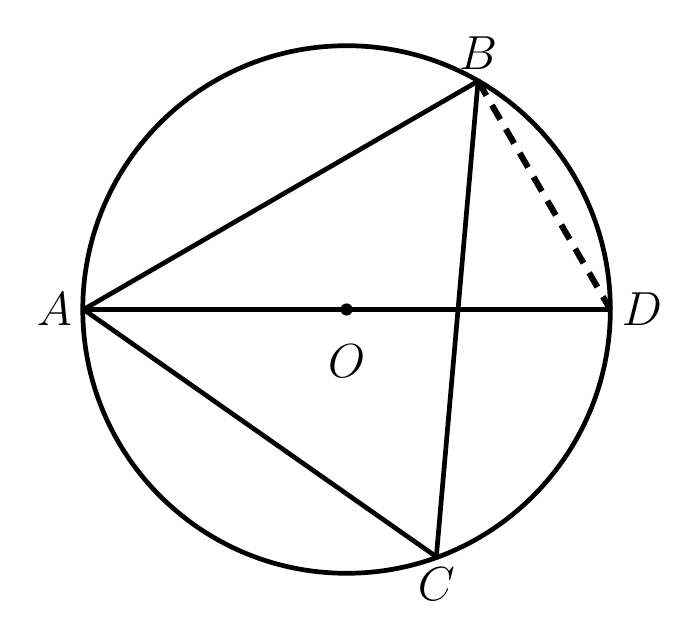
\begin{tikzpicture}[line join=round, line width=1.7pt]
  % Coordinates in cm: s = 0.021277 cm/px, origin at circle centre O (y up)
  \coordinate (O) at (0,0);
  \coordinate (A) at (-3.34,0);   % left end of diameter
  \coordinate (D) at (3.35,0);    % right end of diameter
  \coordinate (B) at (1.67,2.90); % upper-right point on circle
  \coordinate (C) at (1.14,-3.14);% lower-right point on circle

  % Circle, radius 157.24 px * s = 3.35 cm
  \draw (O) circle (3.35);

  % Solid segments: AB, AC, BC (crosses AD unlabelled), diameter AD
  \draw (A) -- (B);
  \draw (A) -- (C);
  \draw (B) -- (C);
  \draw (A) -- (D);

  % Dashed chord BD: longer dashes, slightly heavier stroke
  \draw[dash pattern=on 6pt off 4pt, line width=2.2pt] (B) -- (D);

  % Filled dot at the centre O (radius about 2.2 pt)
  \fill (O) circle (2.2pt);

  % Labels (italic math, 17.5 pt font)
  \node[left,  font=\fontsize{17.5}{21}\selectfont] at (A) {$A$};
  \node[right, font=\fontsize{17.5}{21}\selectfont] at (D) {$D$};
  \node[above, font=\fontsize{17.5}{21}\selectfont] at (B) {$B$};
  \node[below, font=\fontsize{17.5}{21}\selectfont] at (C) {$C$};
  % O label pushed further below the centre
  \node[below, yshift=-0.3cm, font=\fontsize{17.5}{21}\selectfont] at (O) {$O$};
\end{tikzpicture}
\end{document}